%%% Local Veriables:
%%% coding: utf-8
%%% mode: latex
%%% TeX-engine: xetex
%%% End:

\documentclass{article}
\usepackage{latexsym}
\usepackage{amsmath}
\usepackage{amssymb}


\usepackage{xeCJK}
\usepackage{fontspec,xltxtra,xunicode}
\setCJKmainfont[ItalicFont=KaiTi, BoldFont=SimHei]{SimSun}
\setCJKsansfont{SimHei}
\setCJKmonofont{FangSong}

\newcommand{\song}{\CJKfamily{SimSun}}
\setCJKfamilyfont{fs}{FangSong}
\newcommand{\fs}{\CJKfamily{fs}}
\setCJKfamilyfont{kai}{KaiTi}
\newcommand{\kai}{\CJKfamily{kai}}
\setCJKfamilyfont{yahei}{Microsoft YaHei}
\newcommand{\yahei}{\CJKfamily{yahei}}
\setCJKfamilyfont{hei}{SimHei}
\newcommand{\hei}{\CJKfamily{hei}}
\setCJKfamilyfont{lishu}{LiSu}
\newcommand{\lishu}{\CJKfamily{lishu}}
\setCJKfamilyfont{youyuan}{YouYuan}
\newcommand{\youyuan}{\CJKfamily{youyuan}}

\usepackage{graphicx}

\begin{document}
\author{BYIII}
\title{AXIS, ANGLE \& Rotation Matrix}
\date{}

\maketitle

\section{Composition of Rotation Matrix}
\textbf{Problem:} Given rotation axis, a rotation angle, generate the corresponding rotation atrix.

\begin{figure}[!h]
\centering
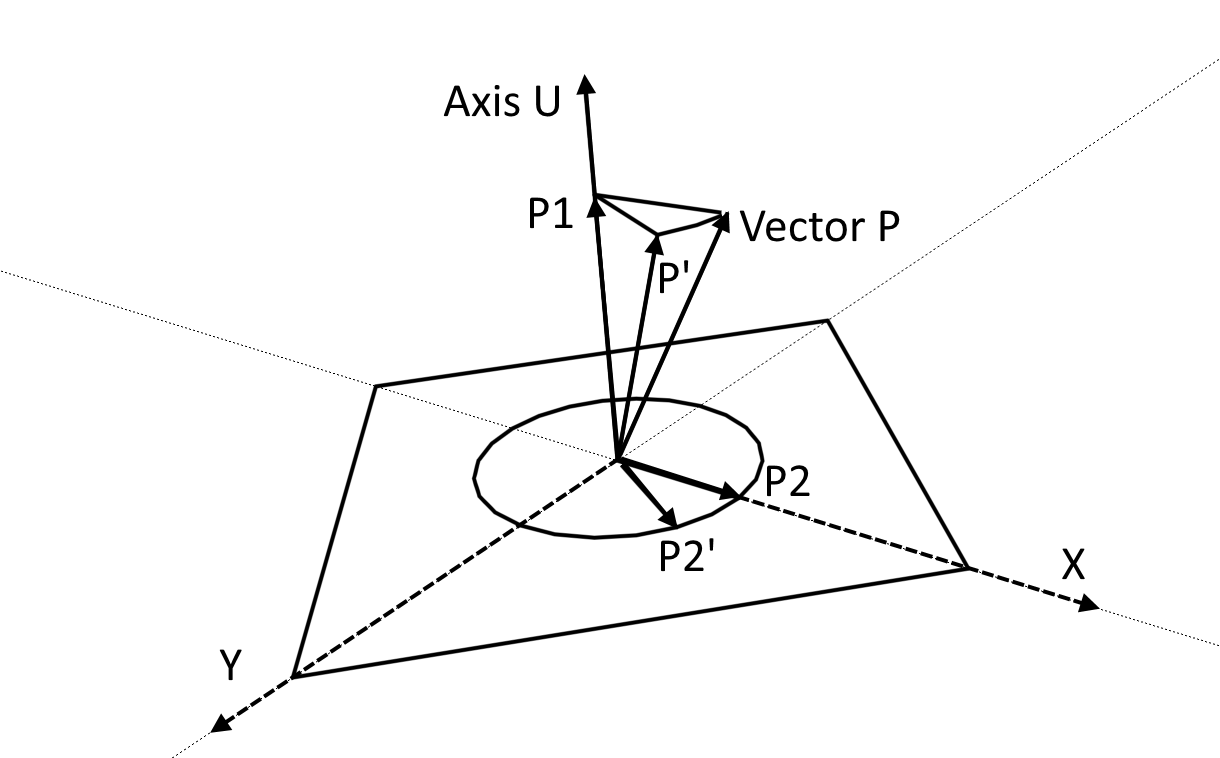
\includegraphics[width=3in]{figures/axis_angle_rot3.png}
\caption{Rotating a vector P about the axis U}
\label{fig1}
\end{figure}

\textbf{Solution}


As show in Figure \ref{fig1}, the axis \textbf{U} goes through the origin, a vector \textbf{P} rotates about \textbf{U} to $\mathbf{P}'$. Let $\theta$ denotes the rotation angle, and let $\phi$ denotes the angle between \textbf{U} and \textbf{P}. From \textbf{U} we can define a plane $S$(whose normal is \textbf{U}). Now we have: 
\begin{displaymath}
\begin{split}
\mathbf{U} &= [u_x, u_y, u_z]^T, \\
&  u_x^2+u_y^2+u_z^2 = 1, \\
\mathbf{P} &= [x, y, z]^T, \\
\mathbf{P}' &= [x', y', z']^T.
\end{split}
\end{displaymath}

Project \textbf{P} to \textbf{U} and $S$, we can get $\mathbf{P}_1$ and $\mathbf{P}_2$:
\begin{displaymath}
\begin{split}
\mathbf{P} &= \mathbf{P}_1+\mathbf{P}_2, \\
\mathbf{P}_1 &= (\mathbf{P}\cdot\mathbf{U})\mathbf{U}, \\
|\mathbf{P}_1| &=  |\mathbf{P}|\cos{\phi}, \\
\mathbf{P}_2 &= \mathbf{P} - \mathbf{P}_1, \\
|\mathbf{P}_2| &=  |\mathbf{P}|\sin{\phi}.
\end{split}
\end{displaymath}

Notice that rotating \textbf{P} is equivalent to firstly rotating $\mathbf{P}_2$ a $\theta$ angle to $\mathbf{P}'_2$ and then combining $\mathbf{P}_1$ and $\mathbf{P}'_2$ to form $\mathbf{P}'$. So, next step is to determine $\mathbf{P}'_2$. 

To represent $\mathbf{P}'_2$, we first to establish some frame for plane $S$. It is convenient to choose vector $\mathbf{P}_2$ be the \textit{unit vector}(though, maybe $|\mathbf{P}_2| \ne 1$) of the X axis, and some other vector $\mathbf{P}_3$ with the same length of $\mathbf{P}_2$ as the Y axis of plane $S$, which satisfies
\begin{displaymath}
\begin{split}
\mathbf{P}_2 \cdot \mathbf{P}_3 = 0, \\
|\mathbf{P}_2| = |\mathbf{P}'_2| = |\mathbf{P}_3|.
\end{split}
\end{displaymath}
Now, according to the rotation matrix in 2D plane, we can write:
\begin{displaymath}
\mathbf{P}'_2 = \mathbf{P}_2\cos{\theta} + \mathbf{P}_3\sin{\theta}.
\end{displaymath}
Then, we determine $\mathbf{P}_3$. It is true that $\mathbf{P}_3$ is parallel to $\mathbf{P}\times\mathbf{U}$, and 
\begin{displaymath}
|\mathbf{P}\times\mathbf{U}| = |\mathbf{P}| \cdot 1 \cdot \sin{\phi} = |\mathbf{P}_2| = |\mathbf{P}_3|.
\end{displaymath}
So we can get:
\begin{displaymath}
\mathbf{P}_3 = \mathbf{P}\times\mathbf{U}.
\end{displaymath}

Combining above:
\begin{displaymath}
\begin{split}
\mathbf{P}' &= \mathbf{P}_1 + \mathbf{P}'_2 \\
 &= (\mathbf{P}\cdot\mathbf{U})\mathbf{U} + [\mathbf{P}-(\mathbf{P}\cdot\mathbf{U})\mathbf{U}]\cos{\theta}+\mathbf{P}\times\mathbf{U}\sin{\theta} \\
 &= \mathbf{P}\cos{\theta} + (\mathbf{P}\cdot\mathbf{U})\mathbf{U}(1-\cos{\theta})+\mathbf{P}\times\mathbf{U}\sin{\theta}
\end{split}
\end{displaymath}
Therefore, the rotatio matrix is
\begin{displaymath}
\end{displaymath}

\section{Decomposition}

\end{document}
